\section{Referencia de la Clase Tipo\-Articulo\-List}
\label{classTipoArticuloList}\index{TipoArticuloList@{TipoArticuloList}}
Muestra y administra la ventana con la informaci\'{o}n de un tipo de art\'{\i}culo.  


{\tt \#include $<$tiposarticuloview.h$>$}

Diagrama de colaboraci\'{o}n para Tipo\-Articulo\-List:\begin{figure}[H]
\begin{center}
\leavevmode
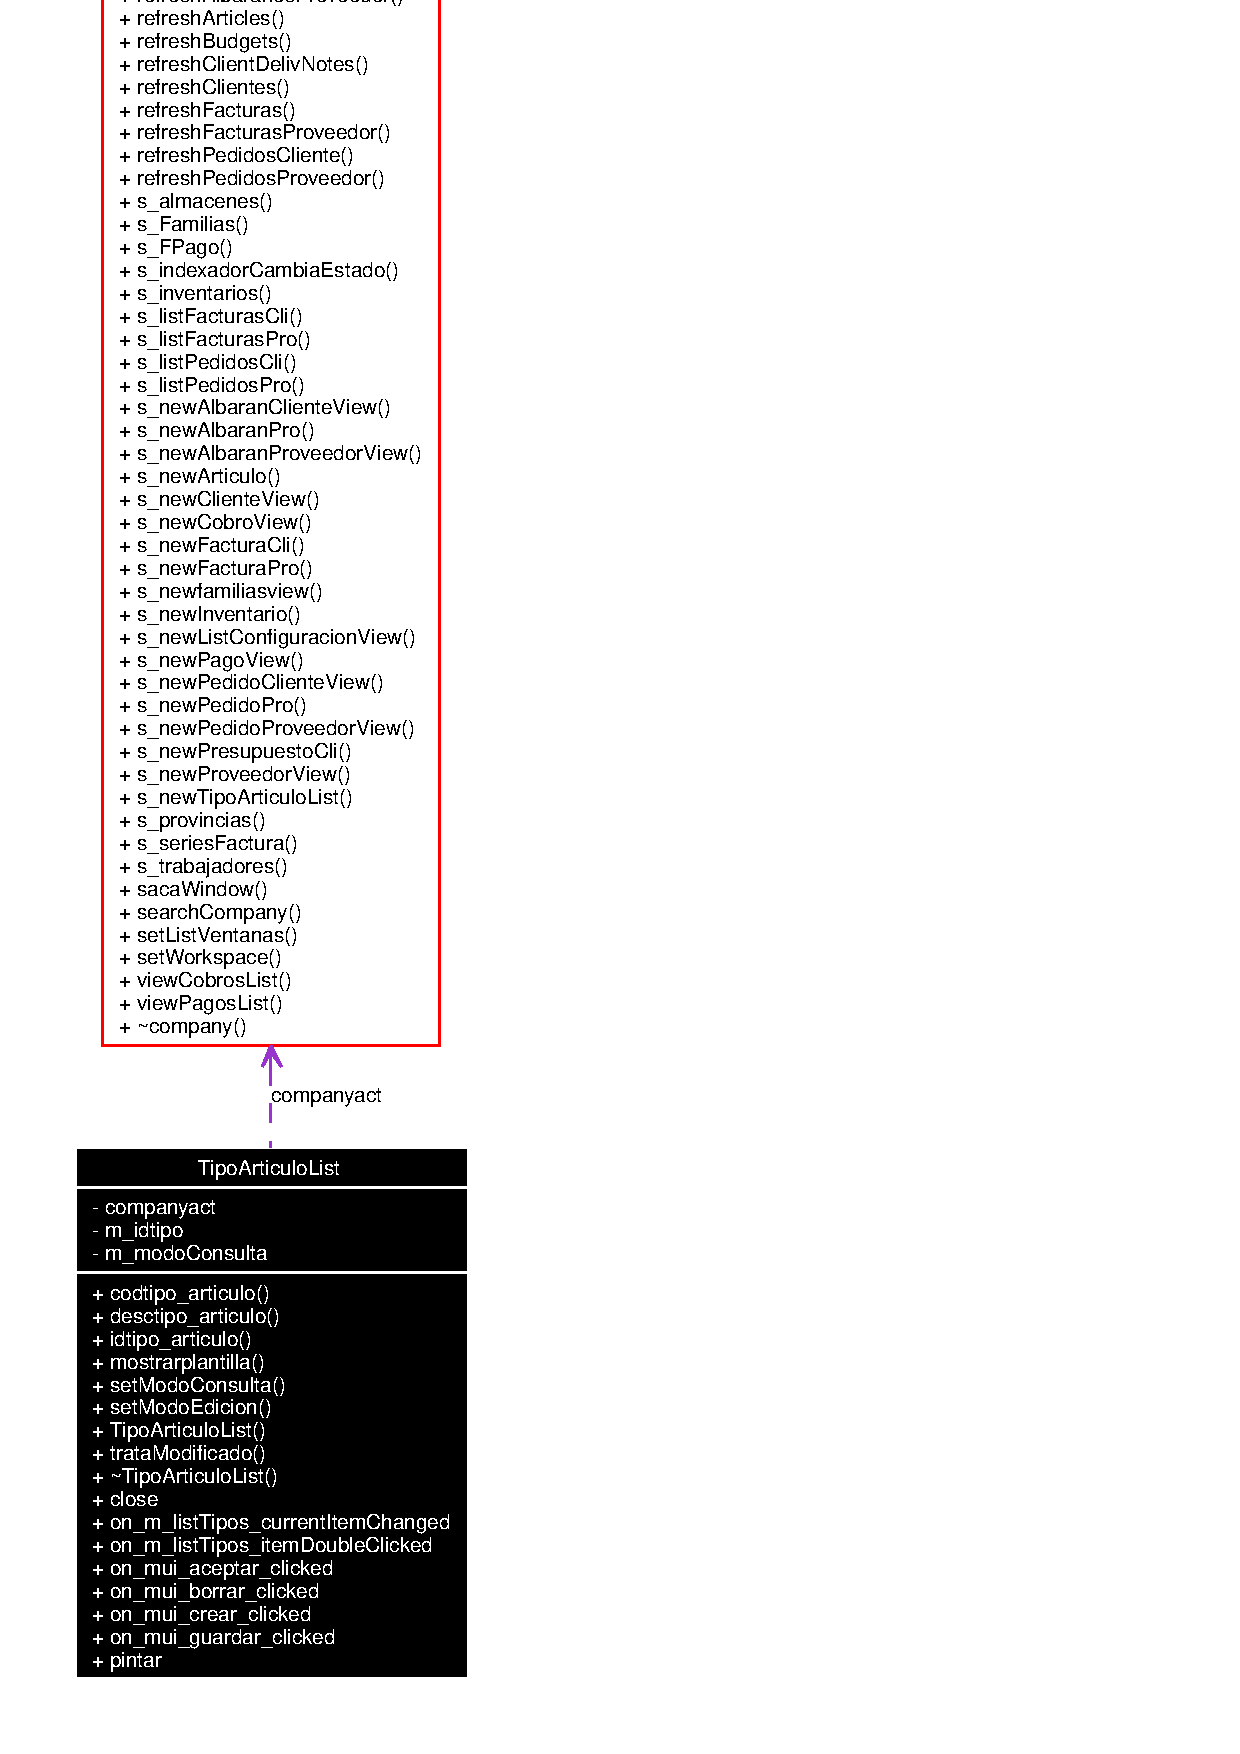
\includegraphics[width=112pt]{classTipoArticuloList__coll__graph}
\end{center}
\end{figure}
\subsection*{Slots p\'{u}blicos}
\begin{CompactItemize}
\item 
virtual void {\bf close} ()
\item 
virtual void {\bf on\_\-m\_\-list\-Tipos\_\-current\-Item\-Changed} (QTree\-Widget\-Item $\ast$current, QTree\-Widget\-Item $\ast$previous)
\item 
virtual void {\bf on\_\-m\_\-list\-Tipos\_\-item\-Double\-Clicked} (QTree\-Widget\-Item $\ast$item, int column)
\item 
virtual void {\bf on\_\-mui\_\-aceptar\_\-clicked} ()\label{classTipoArticuloList_i3}

\item 
virtual void {\bf on\_\-mui\_\-borrar\_\-clicked} ()
\item 
virtual void {\bf on\_\-mui\_\-crear\_\-clicked} ()
\item 
virtual void {\bf on\_\-mui\_\-guardar\_\-clicked} ()
\item 
virtual void {\bf pintar} ()
\end{CompactItemize}
\subsection*{Se\~{n}ales}
\begin{CompactItemize}
\item 
void {\bf selected} (QString)\label{classTipoArticuloList_l0}

\end{CompactItemize}
\subsection*{M\'{e}todos p\'{u}blicos}
\begin{CompactItemize}
\item 
QString {\bf codtipo\_\-articulo} ()\label{classTipoArticuloList_a0}

\item 
QString {\bf desctipo\_\-articulo} ()\label{classTipoArticuloList_a1}

\item 
QString {\bf idtipo\_\-articulo} ()\label{classTipoArticuloList_a2}

\item 
void {\bf mostrarplantilla} ()
\item 
void {\bf set\-Modo\-Consulta} ()\label{classTipoArticuloList_a4}

\item 
void {\bf set\-Modo\-Edicion} ()\label{classTipoArticuloList_a5}

\item 
{\bf Tipo\-Articulo\-List} ({\bf company} $\ast$, QWidget $\ast$parent=0, bool modo\-Consulta=FALSE)\label{classTipoArticuloList_a6}

\item 
bool {\bf trata\-Modificado} ()
\end{CompactItemize}


\subsection{Descripci\'{o}n detallada}
Muestra y administra la ventana con la informaci\'{o}n de un tipo de art\'{\i}culo. 



\subsection{Documentaci\'{o}n de las funciones miembro}
\index{TipoArticuloList@{Tipo\-Articulo\-List}!close@{close}}
\index{close@{close}!TipoArticuloList@{Tipo\-Articulo\-List}}
\subsubsection{\setlength{\rightskip}{0pt plus 5cm}void Tipo\-Articulo\-List::close ()\hspace{0.3cm}{\tt  [virtual, slot]}}\label{classTipoArticuloList_i0}


Antes de salir de la ventana debemos hacer la comprobacion de si se ha modificado algo Esta funcion esta dedicada a Francina, Bienvenida al mundo \index{TipoArticuloList@{Tipo\-Articulo\-List}!mostrarplantilla@{mostrarplantilla}}
\index{mostrarplantilla@{mostrarplantilla}!TipoArticuloList@{Tipo\-Articulo\-List}}
\subsubsection{\setlength{\rightskip}{0pt plus 5cm}void Tipo\-Articulo\-List::mostrarplantilla ()}\label{classTipoArticuloList_a3}


Comprobamos cual es la cadena inicial. \index{TipoArticuloList@{Tipo\-Articulo\-List}!on_m_listTipos_currentItemChanged@{on\_\-m\_\-listTipos\_\-currentItemChanged}}
\index{on_m_listTipos_currentItemChanged@{on\_\-m\_\-listTipos\_\-currentItemChanged}!TipoArticuloList@{Tipo\-Articulo\-List}}
\subsubsection{\setlength{\rightskip}{0pt plus 5cm}void Tipo\-Articulo\-List::on\_\-m\_\-list\-Tipos\_\-current\-Item\-Changed (QTree\-Widget\-Item $\ast$ {\em current}, QTree\-Widget\-Item $\ast$ {\em previous})\hspace{0.3cm}{\tt  [virtual, slot]}}\label{classTipoArticuloList_i1}


Se ha seleccionado un item en la lista Lo que hacemos es mostar el elemento Si el anterior ha sido modificado pedimos para actuar en consecuencia.

Si usamos el trata\-Modificado peta porque si se guarda se sobreescribe el puntero it. \index{TipoArticuloList@{Tipo\-Articulo\-List}!on_m_listTipos_itemDoubleClicked@{on\_\-m\_\-listTipos\_\-itemDoubleClicked}}
\index{on_m_listTipos_itemDoubleClicked@{on\_\-m\_\-listTipos\_\-itemDoubleClicked}!TipoArticuloList@{Tipo\-Articulo\-List}}
\subsubsection{\setlength{\rightskip}{0pt plus 5cm}void Tipo\-Articulo\-List::on\_\-m\_\-list\-Tipos\_\-item\-Double\-Clicked (QTree\-Widget\-Item $\ast$ {\em item}, int {\em column})\hspace{0.3cm}{\tt  [virtual, slot]}}\label{classTipoArticuloList_i2}


Se ha seleccionado un item en la lista Lo que hacemos es mostar el elemento Si el anterior ha sido modificado pedimos para actuar en consecuencia. \index{TipoArticuloList@{Tipo\-Articulo\-List}!on_mui_borrar_clicked@{on\_\-mui\_\-borrar\_\-clicked}}
\index{on_mui_borrar_clicked@{on\_\-mui\_\-borrar\_\-clicked}!TipoArticuloList@{Tipo\-Articulo\-List}}
\subsubsection{\setlength{\rightskip}{0pt plus 5cm}void Tipo\-Articulo\-List::on\_\-mui\_\-borrar\_\-clicked ()\hspace{0.3cm}{\tt  [virtual, slot]}}\label{classTipoArticuloList_i4}


SLOT que responde a la pulsacion del boton de borrar la familia que se esta editando. Lo que hace es que se hace un update de todos los campos. \index{TipoArticuloList@{Tipo\-Articulo\-List}!on_mui_crear_clicked@{on\_\-mui\_\-crear\_\-clicked}}
\index{on_mui_crear_clicked@{on\_\-mui\_\-crear\_\-clicked}!TipoArticuloList@{Tipo\-Articulo\-List}}
\subsubsection{\setlength{\rightskip}{0pt plus 5cm}void Tipo\-Articulo\-List::on\_\-mui\_\-crear\_\-clicked ()\hspace{0.3cm}{\tt  [virtual, slot]}}\label{classTipoArticuloList_i5}


SLOT que responde a la pulsacion del boton de nuevo tipo de iva Inserta en la tabla de ivas

Si se ha modificado el contenido advertimos y guardamos. \index{TipoArticuloList@{Tipo\-Articulo\-List}!on_mui_guardar_clicked@{on\_\-mui\_\-guardar\_\-clicked}}
\index{on_mui_guardar_clicked@{on\_\-mui\_\-guardar\_\-clicked}!TipoArticuloList@{Tipo\-Articulo\-List}}
\subsubsection{\setlength{\rightskip}{0pt plus 5cm}void Tipo\-Articulo\-List::on\_\-mui\_\-guardar\_\-clicked ()\hspace{0.3cm}{\tt  [virtual, slot]}}\label{classTipoArticuloList_i6}


SLOT que responde a la pulsacion del boton de guardar el tipo de iva que se esta editando. Lo que hace es que se hace un update de todos los campos

Vamos a hacer algo no reentrante. \index{TipoArticuloList@{Tipo\-Articulo\-List}!pintar@{pintar}}
\index{pintar@{pintar}!TipoArticuloList@{Tipo\-Articulo\-List}}
\subsubsection{\setlength{\rightskip}{0pt plus 5cm}void Tipo\-Articulo\-List::pintar ()\hspace{0.3cm}{\tt  [virtual, slot]}}\label{classTipoArticuloList_i7}


vaciamos el arbol.

Comprobamos cual es la cadena inicial. \index{TipoArticuloList@{Tipo\-Articulo\-List}!trataModificado@{trataModificado}}
\index{trataModificado@{trataModificado}!TipoArticuloList@{Tipo\-Articulo\-List}}
\subsubsection{\setlength{\rightskip}{0pt plus 5cm}bool Tipo\-Articulo\-List::trata\-Modificado ()}\label{classTipoArticuloList_a7}


Si se ha modificado el contenido advertimos y guardamos. 

La documentaci\'{o}n para esta clase fu\'{e} generada a partir de los siguientes archivos:\begin{CompactItemize}
\item 
tiposarticuloview.h\item 
tiposarticuloview.cpp\end{CompactItemize}
